\chapter{The rewrite}
\label{chap:rewrite}

\section{Principles}

\paragraph{Physical, not pixel, parameters} The first rule I set was to state every length, area and
volume of the configuration in physical units. They are expressed in \um, \umsq{} or \umcube, and converted to pixels once, from the voxel size
(\code{acquisition.}\allowbreak\code{voxel\_size\_um}). Anisotropic voxels are supported: in-plane kernels become
ellipses, 3D neighbourhoods become balls made of per-slice ellipses. Changing the resolution, or
scanning another species, means stating anatomically meaningful sizes, not re-tuning pixel counts.
I build the kernels analytically: OpenCV's elliptic structuring elements carry one-pixel spikes at
their tips, and a one-row ``ellipse'' degenerates to a single pixel.

\paragraph{Decisions from physics} Wherever our 2018 code set a boundary with a morphological radius, I
derived it instead from how the scanner forms the image: a global intensity model, partial-volume
edges at half-maximum, densities rather than dilated masks. I removed the operations that can invent
shapes (closing, dilation by a fixed radius); the remaining ones only keep or drop whole components
(area filters, morphological reconstruction, hole filling).

\paragraph{Measured} I kept no change unless it improved the score on a ground truth
(Chapter~\ref{chap:validation}) and looked right on the real data.

\section{Architecture}

The package is split by responsibility:
\begin{center}
\small
\begin{tabularx}{0.92\linewidth}{@{}lX@{}}
\toprule
\code{config/}        & JSON defaults, pydantic schema (types, bounds, what a change affects, when
                        to change it), loader with overrides \\
\code{io/}            & slice stacks read lazily from a directory or straight from the zip,
                        streamed \code{.npy} volumes, image-sequence export (ImageJ) \\
\code{imaging/}       & binary morphology, multi-Otsu, Gaussian-derivative Hessian, eigenvalues \\
\code{segmentation/}  & classifier, bursts, tubularity, 3D connectivity, refinement, pipeline \\
\code{meshing/}       & marching cubes, Taubin smoothing, STL and glTF files \\
\code{quantification/} & cavities, centrelines and wall distances (interchangeable backends),
                        network graph, pruning, measures (Chapter~\ref{chap:network}) \\
\code{analysis/}, \code{visualization/} & agreement metrics, label overlays \\
\code{cli/}           & the \code{pybones} command (also \code{python -m pybones}); arguments
                        validated into one typed model per sub-command \\
\code{api/}           & every operation as a plain function; background jobs with progress,
                        cancellation and pushed status events \\
\code{server/}        & the local web server (FastAPI) and the web page it serves \\
\code{utils/}         & logging (one file per run), the ordered thread map, sliding windows along
                        $z$, format constants \\
\code{tools/}         & annotation page, synthetic phantom, report benchmark and figures \\
\bottomrule
\end{tabularx}
\end{center}

\paragraph{Streaming} The stack is never held in memory. Slices are decoded a few at a time,
classified in a thread pool, and the label volume is written slice by slice to a \code{.npy} file
(one byte per voxel, values \code{background}, \code{bone}, \code{vessel}, \code{burst}). Every step
that needs neighbouring slices works on a sliding window along $z$, mirrored at the ends of the stack.
The threads pay off because OpenCV, zlib and most numpy kernels release Python's global lock: when I
measured it on the reference stack, the per-slice stage ran about twice as fast with 4 threads as
sequentially, for about fifteen lines of code (an ordered map with a bounded number of pending jobs).

\paragraph{Configuration} Every tunable value lives in one JSON file, validated by a strict pydantic
schema: unknown keys are rejected, every number has bounds, label-keyed maps must be complete. A user
file only states what it changes; single values can be overridden on the command line
(\code{--set segmentation.burst.density=0.3}). The effective configuration is stored in the
\code{meta.json} of every segmentation, with the thresholds, statistics, timings and version.

\paragraph{Quality} I held the code to explicit conventions: no magic numbers or strings (configuration
or named constants), complete Google-style docstrings with type hints on every function, imports used
only in annotations under \code{if TYPE\_CHECKING:}, no imports inside functions. Ruff, basedpyright and
a dedicated test enforce them; two more tests reject duplicated code and dead code (a definition
nothing but the tests uses). A pytest suite checks every algorithm on synthetic data, most of them
against brute-force reference implementations (flood fill for 3D connectivity, \code{numpy.linalg} for
the eigenvalues, loops for multi-Otsu and the majority vote). A ``golden'' regression test segments a
small, fixed phantom and compares its scores with a recorded baseline: a change of any score, up or
down, must be deliberate.

\paragraph{Programmatic interface} Every operation (segment, preview, mesh, export, compare, quantify) is a plain
function of \code{pybones.api}, which the command line merely wraps. Long runs can be started as
background jobs that report their progress (stage, overall fraction, remaining time) and can be
cancelled, leaving no partial file behind. Every run also writes its own log file.

\paragraph{Web server} \code{pybones serve} puts an HTTP interface (FastAPI) on top of these functions.
It lists the stacks of a data folder and the segmentations of an output folder, starts segmentations,
meshes and quantifications as background jobs whose progress is pushed to the browser as it happens
(Server-Sent Events, no polling), renders a slice with its labels, and serves the meshes and the
measured network. A client only names things
by their id, never by a path, so no request can reach another file. Its settings (address, folders)
are kept apart from the segmentation configuration, which every segmentation records with its result.

\paragraph{Web page} The same server serves a page (Figure~\ref{fig:webpage}) that does what the 2018
viewer did, in a browser: segment a stack and follow the run, scroll through its slices with the labels
overlaid, turn its meshes around in 3D, measure its vessel network (Chapter~\ref{chap:network}), and
compare it with another run (Figure~\ref{fig:compare}): the settings that differ, the results side
by side and the same slice of both.
It is plain HTML, CSS and JavaScript modules, with no build
step; the 3D view uses three.js, kept in the repository at a fixed version with the hash of each file,
so that the page works offline and changes only on purpose. A mesh is sent to the browser once as GLB
(Section~\ref{sec:meshing}) and drawn by the graphics card: rotating it costs no request. Each kind of job
has a settings form built from the configuration's schema (a run's, the meshes', the network's): each
setting says what it is, when to change it and what a change affects (the labels, and so the meshes
and the network; the meshes or the network only; or no result, such as the number of threads);
values are checked as typed, and the server's own refusals come back next to their setting. A job
changes its own section only, and records what it used: a mesh writes its settings next to it, a
network inside its file, so the page can say when a mesh was built with other settings than its
form's. A run can be started again from the one on screen, with its settings filled in, and the form
then says what differs from it. Every section of the configuration declares what a change of it
affects, and a test refuses a new one that does not. Each step of the page was checked
in Firefox, and the tests check that every module it imports is served and every name it imports
exists; with Node.js installed, they also run unit tests of its helpers and of its HTTP client, and
check that its labels, job states, job kinds, effects and levels match the Python ones, and that
each settings form reads exactly the settings its job may change. The page's own files are
served with \code{no-cache}: the browser keeps them but checks them on every load, so an updated
module never meets an old one. Chapter~\ref{chap:performance} describes how it keeps the browser's memory bounded.

\begin{figure}[ht]
  \centering
  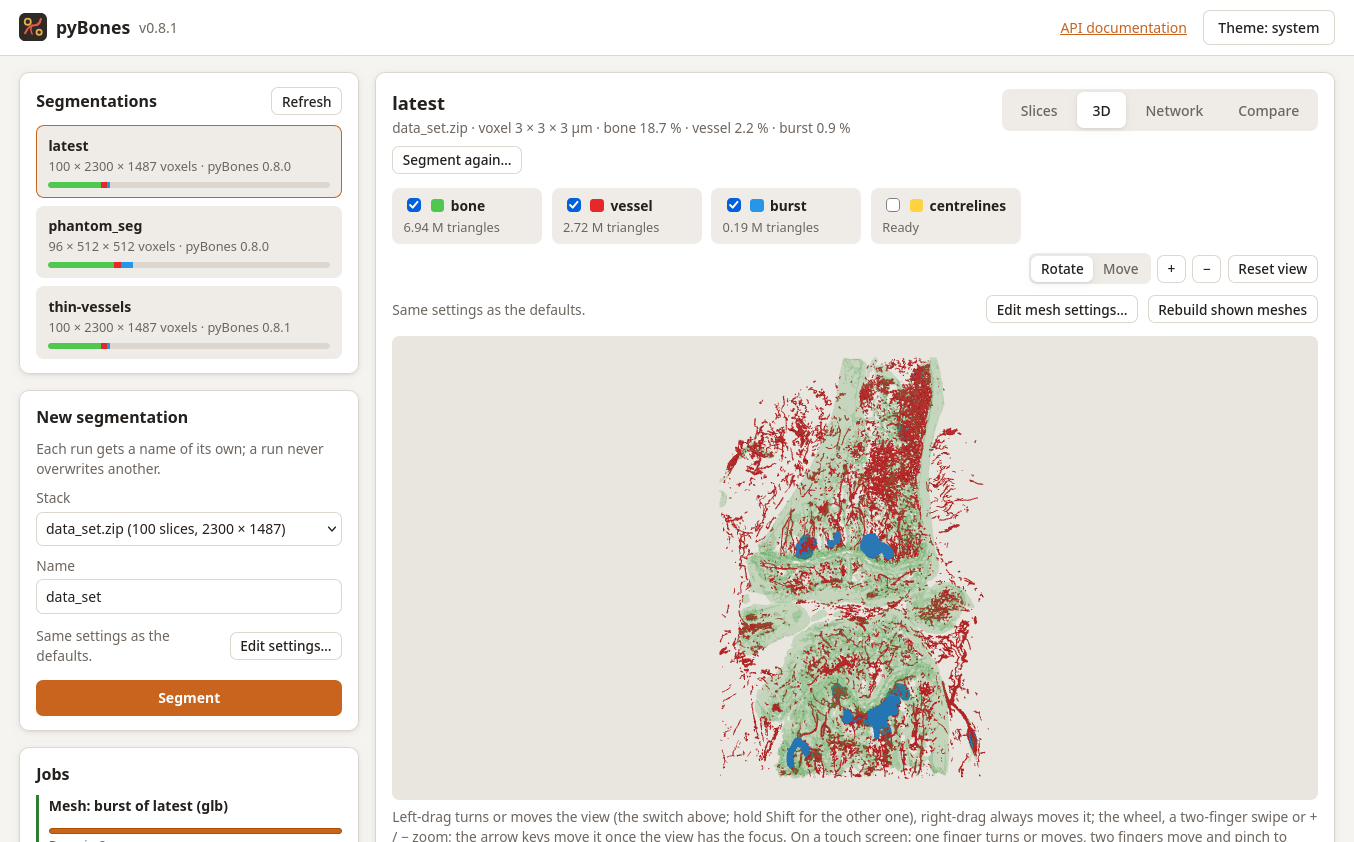
\includegraphics[width=\linewidth]{../../screenshots/06-web-page.png}
  \caption{The web page: segmentations and the jobs that built the meshes on the left; the meshes of
    the whole stack on the right, bone see-through, vessels in red, bursts in blue.}
  \label{fig:webpage}
\end{figure}

\begin{figure}[ht]
  \centering
  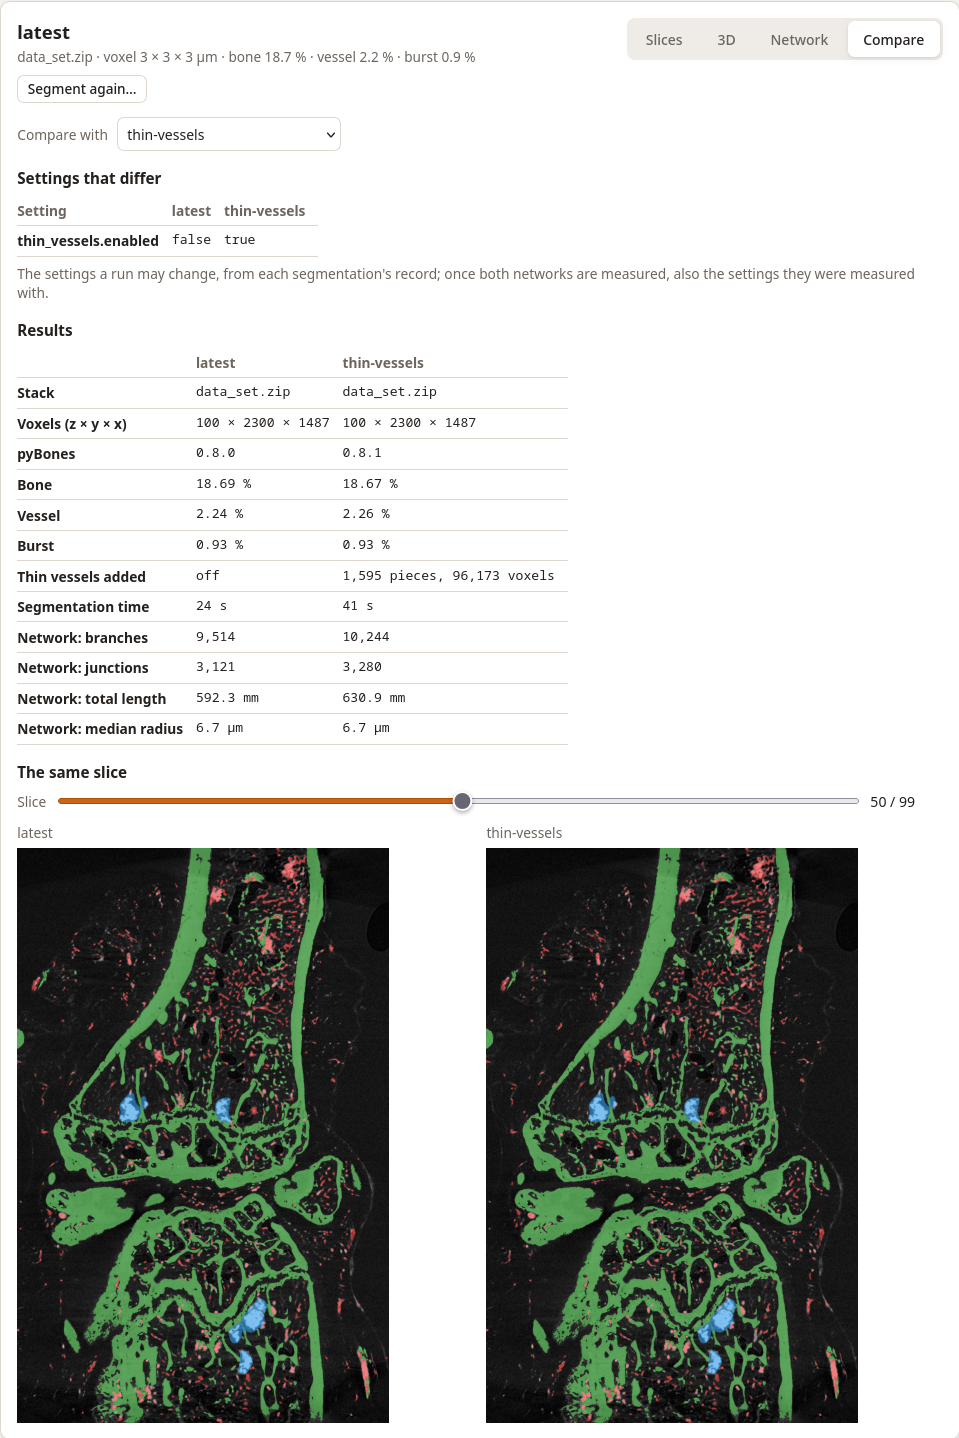
\includegraphics[width=0.75\linewidth]{../../screenshots/08-compare.png}
  \caption{The Compare tab: the sample segmented without and with the optional thin-vessel pass
    (Section~\ref{sec:thinvessels}): the setting that differs, the results side by side, and the
    same slice of both.}
  \label{fig:compare}
\end{figure}

\section{Pipeline}

\begin{figure}[ht]
\centering
\begin{tikzpicture}[
  node distance=5mm and 7mm,
  box/.style={draw=accent,line width=0.7pt,rounded corners=2pt,fill=accent!6,align=center,
              minimum height=11mm,text width=29mm,font=\small},
  data/.style={draw=muted,rounded corners=2pt,fill=white,align=center,minimum height=9mm,
               text width=26mm,font=\small},
  arrow/.style={-{Latex[length=2mm]},line width=0.7pt,color=ink}]
  \node[data] (zip) {slices\\\footnotesize(zip or folder)};
  \node[box, right=of zip] (thr) {global thresholds\\\footnotesize 3-class Otsu};
  \node[box, right=of thr] (cls) {per-slice classes\\\footnotesize z window, threaded};
  \node[box, below=of cls] (burst) {bursts\\\footnotesize 3D density, streamed};
  \node[box, left=of burst] (tube) {tubularity\\\footnotesize 3D Hessian};
  \node[box, left=of tube] (ref) {3D refinement\\\footnotesize union-find, 3 passes;\\\footnotesize then thin vessels\\\footnotesize (optional)};
  \node[data, below=of ref] (vol) {\code{labels.npy}\\\code{meta.json}};
  \node[box, right=of vol] (mesh) {meshing\\\footnotesize marching cubes, Taubin};
  \node[data, right=of mesh] (stl) {STL, GLB,\\PNG sequences};
  \node[box, below=of mesh] (net) {vascular network\\\footnotesize skeleton, graph, pruning};
  \node[data, right=of net] (netfiles) {\code{network.json},\\\code{branches.csv}, centrelines};
  \draw[arrow] (zip) -- (thr);
  \draw[arrow] (thr) -- (cls);
  \draw[arrow] (cls) -- (burst);
  \draw[arrow] (burst) -- (tube);
  \draw[arrow] (tube) -- (ref);
  \draw[arrow] (ref) -- (vol);
  \draw[arrow] (vol) -- (mesh);
  \draw[arrow] (mesh) -- (stl);
  \draw[arrow] (vol) |- (net);
  \draw[arrow] (net) -- (netfiles);
\end{tikzpicture}
\caption{The pyBones pipeline. Only the boxes in the first two rows touch the raw data; each of them
  streams the stack slice by slice (or through a short window of slices).}
\label{fig:pipeline}
\end{figure}

\begin{enumerate}
  \item \textbf{Thresholds}: one 3-class Otsu for the whole stack (Section~\ref{sec:thresholds}).
  \item \textbf{Per-slice classification}: bright cores and their partial-volume rims are vessels,
        large bone-intensity regions are bone, small ones are marked \emph{ambiguous}
        (Section~\ref{sec:edges}).
  \item \textbf{Bursts}: dense clusters of bright pixels, measured per slice and in a 3D box
        (Section~\ref{sec:bursts}).
  \item \textbf{Tubularity}: a tube-versus-plate measure for every ambiguous voxel
        (Section~\ref{sec:tubularity}).
  \item \textbf{3D refinement}: each ambiguous 3D blob is decided by what it touches and by its shape;
        3D specks are removed (Section~\ref{sec:refinement}).
  \item \textbf{Thin vessels} (optional, off by default): thin pieces that a deconvolved image shows
        as bright as a vessel become vessel (Section~\ref{sec:thinvessels}).
  \item \textbf{Meshing}: surfaces for any label (Section~\ref{sec:meshing}).
  \item \textbf{Vascular network}: centrelines, a graph of branches and junctions, its measures
        (Chapter~\ref{chap:network}).
\end{enumerate}
